\section{Grundlagen}
Um die Implementierung der Arbeit vollständig nachvollziehen zu können, ist es wichtig, einige Konzepte verstanden zu haben und zu wissen, worauf die Entwicklung aufbauen wird. Diese Grundlagen werden im Folgenden eingeführt werden.

\subsection{Einführung in Frontend-Frameworks für Webapplikationen}
Um interaktive Webapplikationen zu entwickeln, müssen diese mit HTML, CSS und JavaScript programmiert werden. Browser stellen den mit HTML definierten Inhalt dar, manipulieren das Aussehen der Seite anhand der durch CSS definierten Regeln und verfügen zudem über einen \gls{JS} Interpreter, der den übermittelten \gls{JS} Code ausführen kann und darüber eine Manipulation der Seiteninhalte erlauben.

Durch diese Möglichkeit ergibt sich das Problem, dass die Daten, die das Programm berechnet (oder auf andere Weise erlangt) Usern korrekt dargestellt werden und umgekehrt Eingaben von Usern sich in den Daten widerspiegeln sollen.

Beim Entwickeln solcher Funktionalität wiederholen sich häufig bestimmte Probleme wie die Synchronisierung von Daten mit der Anzeige oder die Wiederverwendung von Teilen der Nutzeroberfläche. Diese Probleme können mit Hilfe von Frontend-Frameworks gelöst werden.

Zur Zeit gibt es vor allem drei Frameworks, die häufig verwendet werden: React, Angular und Vue \cite{stateofjs}. Angular baut dabei auf dem klassischen \gls{MVC}-Pattern auf. In einer Variation von HTML, in der bestimmte TypeScript-Ausdrücke interpretiert werden können, kann die View aufgebaut werden. Die Funktionalität des Controllers wird in einer TypeScript-Klasse implementiert und das Model kann über Services dargestellt werden, die dann automatisch instanziiert und in die Controller injected werden. \missingQuote

Vue und React verfolgen nicht so strikt das \gls{MVC}-Pattern. Vue verfügt (ähnlich wie Angular) über eine Variation von HTML, in der auch bestimmte Ausdrücke evaluiert werden können, sodass so die View definiert werden kann. Allerdings ist es bei Vue üblich, dass sich noch in derselben Datei wie die View (und das CSS) auch der Controller befindet. Vue gibt im Gegensatz zu Angular keine klare Vorgabe, wie das Model umzusetzen ist.

React hingegen verfügt über einen anderen Ansatz. Hier wird es ermöglicht, eine Variante von HTML-Ausdrücken in JavaScript bzw. TypeScript einzufügen, die dann wie andere Werte auch in Variablen gespeichert werden können. Auf diesem Weg wird parallel zum eigentlichen \gls{DOM} ein sogenanntes Shadow DOM generiert, der dann in das eigentliche \gls{DOM} überführt wird. Somit ist es in React möglich, View und Controller komplett miteinander zu verbinden. Zudem verfügt auch React nicht über einen klaren Ansatz um das Model umzusetzen.

Alle drei dieser Frameworks ermöglichen eine komponentenbasierte Entwicklung. Das bedeutet, dass mit sehr geringem Aufwand die View in Komponenten unterteilt werden kann, die dann wiederverwendet werden können.

Aus (unter anderen) diesen Gründen werden aktuelle Webapplikationen in der Regel auf Grundlage eines Frontend-Frameworks aufgebaut \missingQuote. Da jedes Frontend aber mehr oder weniger klare Strukturen, Datenflüsse, Syntaxen und vieles mehr vorgibt, ist die Entscheidung eines Frameworks in Bezug auf die Suche weiterer Abhängigkeiten eine sehr folgenschwere Entscheidung.

Beispielsweise ist es nicht möglich, Angular ohne TypeScript oder React ohne ESLint zu verwenden. Sowohl für React als auch für Angular gibt es Komponentenbibliotheken\footnote{Material-UI für React: \url{https://material-ui.com/}; Angular Material: \url{https://material.angular.io/}}, die Google's Material Design System folgen; allerdings sind diese Bibliotheken sehr verschieden, haben unterschiedliche Features und gehen nicht aus demselben Code hervor.

Die Entscheidung eines Frameworks ist daher eine der ersten Entscheidungen, die Entwickelnde beim Einrichten ihrer Projekte treffen müssen. Sie schränkt die weitere Auswahl an Werkzeugen und Bibliotheken ein. Außerdem können, bis auf in besonderen Kontexten wie Micro-Frontends oder WebComponents \missingQuote, nur mit hohem Aufwand oder gar nicht zwei Frameworks zusammen verwendet werden.

\subsection{Ähnliche Projektgeneratoren}
Um das Problem der initialen Projektkonfiguration zu automatisieren oder zumindest zu erleichtern, bieten die drei oben erwähnten Frameworks jeweils ein Programm an, was (unter anderem) zur initialen Erstellung von Projekten mit dem jeweiligen Framework empfohlen wird.

\subsubsection{React}
In der Dokumentation für React wird empfohlen, neue Projekte über das \gls{CLI} \gls{CRA} zu erstellen. Dieses kann per \gls{npm} installiert werden und ist dann in der Lage, den Inhalt eines angegebenen Templates (oder des Standardtemplates) in ein spezifiziertes Verzeichnis zu kopieren. Daraufhin werden die benötigten Abhängigkeiten per \gls{npm} oder mittels eines anderen installierten Paketmanagers (wie z.B. Yarn) installiert.

Dritten ist es möglich, eigene Templates für \gls{CRA} zu erzeugen, die dann wie Erstanbietertemplates zur Erzeugung des neuen Projekts genutzt werden können. Wenn also mittels \gls{CRA} ein Projekt erzeugt werden soll, das bereits mit gewissen Bibliotheken oder Werkzeugen ausgestattet ist, muss dafür dafür zuvor ein entsprechendes Template erstellt worden sein. Die Wahrscheinlichkeit, dass das jedoch passiert ist, sinkt mit der Spezifität der Wünsche.

Die Erstanbietertemplates geben bereits die empfohlene Ordner- und Dateistruktur für React-Projekte vor; durch Drittanbietertemplates kann hiervon aber abgewichen werden. Außerdem installieren die Erstanbietertemplates bereits einige weitere Werkzeuge wie ESLint, Jest (ein Werkzeug zum Schreiben und Ausführen von automatisierten Tests, in der Regel Unit Tests) und die sogenannten react-scripts. Diese sind eine Sammlung von kleinen Skripten und Abhängigkeiten, die Prozesse automatisieren, die für die Entwicklung notwendig sind. Beispielsweise wird so ein Skript zur Verfügung gestellt, welcher einen lokalen Server startet, der den aktuellen Stand der Webapplikation hostet und bei jeder Codeänderung automatisch aktualisiert. Dieser Server gibt zudem auch die Warnungen aus, die ESLint erzeugt.

Außerdem ist es bei der Verwendung dieser Templates mit geringem Aufwand möglich, bestimmte empfohlene Bibliotheken und Werkzeuge nachzurüsten. So gibt es zum Beispiel Anleitungen für die Installation von Prettier oder von CSS Präprozessoren, die aus jeweils einem in der Kommandozeile auszuführenden Befehl bestehen. Für Prettier muss zudem noch eine bestimmte, bereits existierende Datei um einige Zeilen ergänzt werden.

\subsubsection{Angular}
Das Angular-Team stellt das sog. Angular-CLI zur Verfügung, das Entwickelnden beim Programmieren verschiedene wiederkehrende und repetitive Aufgaben abnehmen soll (wie z.B. die Erstellung und Einbindung neuer Komponenten). Neben diesen Aufgaben wird das Tool auch zur Erstellung neuer Angular-Projekte genutzt.

Der Befehl ng new <project-name> führt Nutzende in einen Dialog, bei dem zwei Fragen zur gewünschten Konfiguration des Projektes gestellt werden. Über explizit gesetzte Kommandozeilenoptionen können dann insgesamt Features konfiguriert werden, mit denen das Projekt eingerichtet wird. Diese Features sind jedoch allesamt Angular-intern, d.h. es gibt keine Möglichkeit weitere Libraries oder ähnliches installieren zu lassen, die nicht direkt vom Angular Team kommen. Selbst einige Libraries (z.B. Angular Material), die vom Angular-Team direkt entwickelt werden, sind nicht in diese initiale Projektgenerierung eingebunden.

  \begin{figure}
	\centering
		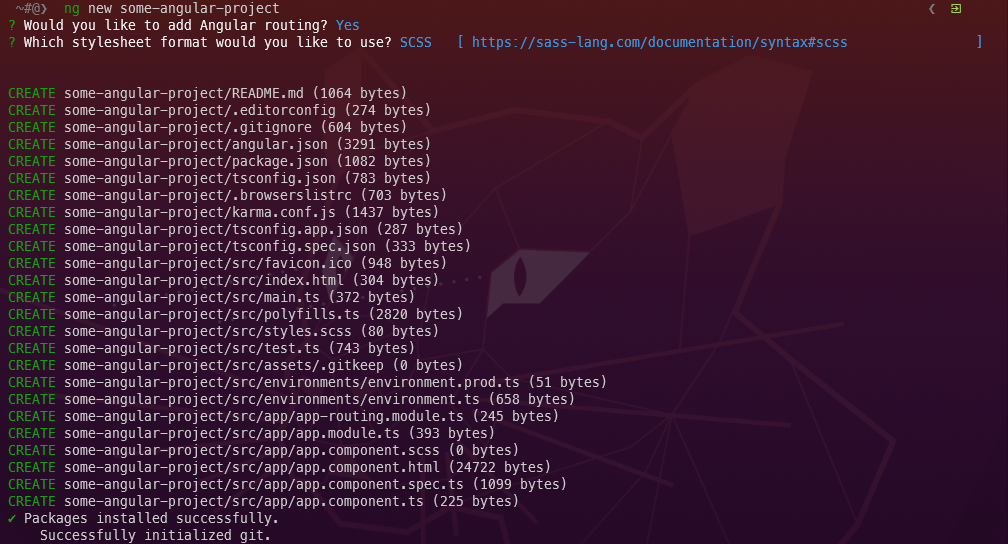
\includegraphics[width=\linewidth]{angular-cli-example.png}
	\caption{Die Ausgabe des Angular CLI's bei der Erzeugung eines neuen Projektes.}
		\label{fig:basics:angular_cli_example}
  \end{figure}

Im Gegensatz zu CRA sind hier die Möglichkeiten, die Nutzenden bei der initialen Projekterstellung geboten werden, sehr eingeschränkt. Es gibt die Möglichkeit, bei der Einrichtung eine sogenannte "Collection" anzugeben, die dann die Erstellung des eigentlichen Projektes übernimmt. Es könnte also eine Collection entwickelt werden, die weitere Libraries je nach Eingabe einbindet. Jedoch scheint die Umsetzung dieses Features abzunehmen: von den überprüften Collections für ESLint, Prettier und Apollo-Angular hat nur eine dieses Feature (also die Installation bei der Initialisierung statt hinterher) jemals unterstützt, hat es aber mittlerweile wieder eingestellt \cite{angular_eslint_collection_issue} \cite{prettier_angular_collection_file} \cite{apollo_angular_collection_file}.

Im Gegensatz zu der React-Lösung können sich Nutzende hier (im Rahmen der beschränkten angebotenen Optionen) eine beliebige Konfiguration aussuchen und sind nicht darauf angewiesen, dass jemand vor ihnen schon denselben Wunsch hatte. Außerdem wird durch die gestellten auch Anfänger:innen die Entdeckung und der Einstieg in Angular erleichtert, da gewisse Features automatisch an sie herangetragen werden.


\subsubsection{Vue}
Von den drei Frameworks bietet Vue in Bezug auf die Projekterstellung das umfangreichste CLI. Zu aller erst besteht die Möglichkeit, ein Preset auszuwählen. Dies kann eines von zwei Standardpresets sein oder eines, was zuvor auf dem lokalen Computer erstellt und gespeichert wurde.

Falls man kein Preset auswählt, trifft man nun zunächst eine Vorauswahl von zehn Features, die man haben oder nicht haben möchte. Daraufhin werden zu den ausgewählten Features detailliertere Fragen gestellt. Insgesamt stehen einem durch dieses Tool über 20 verschiedene Libraries ohne weiteren Konfigurationsaufwand zur Verfügung. Die soeben erstellte Konfiguration kann anschließend als neues Preset gespeichert werden.

  \begin{figure}
		\centering
		\begin{subfigure}[a]{0.4\linewidth}
			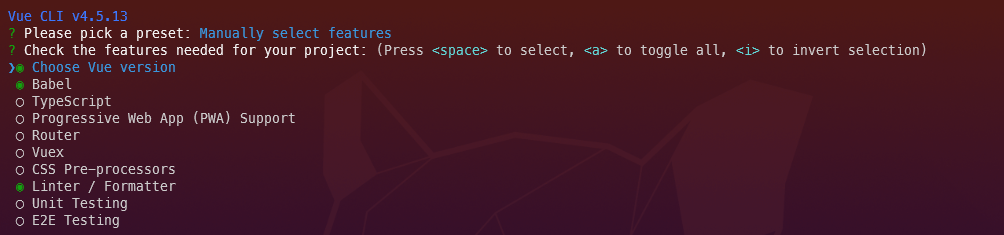
\includegraphics[width=\linewidth]{vue-cli-feature-picker.png}
      		\caption{Das Vue CLI fragt explizit nach zehn verschiedenen Features. Davon kann eine beliebige Teilmenge ausgewählt werden.}
		\end{subfigure}
		\begin{subfigure}[a]{0.4\linewidth}
			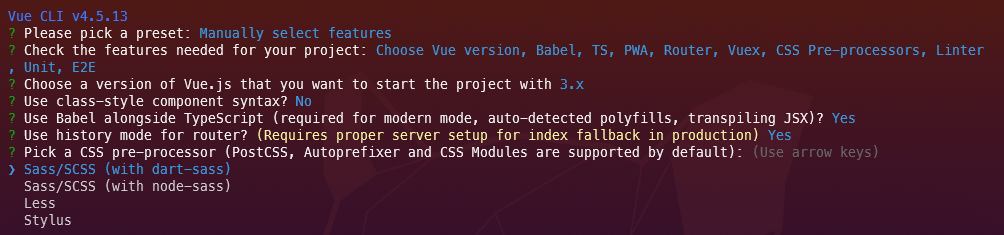
\includegraphics[width=\linewidth]{vue-cli-more-questions.png}
      		\caption{Für jede der Auserwählten Erweiterungen werden Detailliertere Fragen gestellt.}
		\end{subfigure}
		\caption{Zwei Bilder von dem Prozess der Erstellung einer neuen Vue-Applikation.}
		\label{fig:basics:vue_cli_example}
  \end{figure}

%\subsubsection{Vergleich der Möglichkeiten zwischen Frameworks}
%Alle drei Tools bieten Entwickelnden die Möglichkeit, eigene Erweiterungen zu erarbeiten und zu veröffentlichen. Im Falle von React muss dies in Form eines Templates geschehen. Da nur ein Template zur Erstellung eines Projektes genutzt werden kann, sind derartige Erweiterungen hier also exklusiv.

%Bei Angular und React ist es jedoch möglich, auch Erweiterungen zu entwickeln, die zusätzlich zu anderen Optionen und Erweiterungen nutzbar sind. Für das Angular \gls{CLI} kann man sogenannte Schematics entwickeln, die das Hinzufügen und Einbinden einer Bibliothek vollautomatisch übernehmen. Diese Schematics müssen aber leider nach der Installation ausgeführt werden und müssen insbesondere von Nutzenden entdeckt werden. Hierfür gibt es keine eigene Plattform o.ä. und die Auswahl der Schematics, die schon bei der Projekterstellung auswählbar sind, beschränkt sich auf Angular-interne Features (z.B. die Einfügung eines Routers). Selbst Libraries, die auch vom Angular-Team betreut werden (z.B. Angular Material) müssen später per Schematic nachgerüstet werden.

%Im Rahmen des Vue \gls{CLI}'s ist es immerhin möglich, auch Libraries von Dritten direkt bei der Projekterstellung einzubinden. Allerdings ist auch hier die anfängliche Auswahl nicht erweiterbar. Dafür können, wie auch schon bei Angular, anschließend automatisch über Drittanbieterplugins neue Libraries heruntergeladen, importiert und demonstriert werden.

%Tabelle 

%  \begin{table}
%	  \centering
%	  \caption{Automatische und initiale Installierbarkeit verschiedener Features in Angular und Vue Projekten}
%	  \begin{tabular}{|l|l|l|l|l|}
%    \hline
%         & \multicolumn{2}{c|}{Angular} & \multicolumn{2}{c|}{Vue}  \\ \hline
%        Feature & Automatisch & Ititial & Automatisch & Initial \\
%        & installierbar & auswählbar & installierbar & auswählbar \\ \hline
%        TypeScript & \multicolumn{2}{c|}{wird erzwungen} & \checkmark & \checkmark \\ \hline
%        Router & \checkmark & \checkmark & \checkmark & \checkmark \\ \hline
%        PWA-Support & \checkmark & \texttimes & \checkmark & \checkmark \\ \hline
%        Linter & \checkmark & \texttimes & \checkmark & \checkmark \\ \hline
%        Formatierer & \checkmark & \texttimes & \checkmark & \checkmark \\ \hline
%        CSS Reset & \texttimes & \texttimes & \texttimes & \texttimes \\ \hline
%        CSS Präprozessor & \checkmark & \checkmark & \checkmark & \checkmark \\ \hline
%        Design Framework & \checkmark & \texttimes & \checkmark & \texttimes \\ \hline
%        State Management & \multicolumn{2}{c|}{wird erzwungen} & \checkmark & \checkmark %\\ \hline
%        Unit Testing Framework & \checkmark & \texttimes & \checkmark & \checkmark \\ \hline
%        E2E Testing Framework & \checkmark & \texttimes & \checkmark & \checkmark \\ \hline
%    \end{tabular}
%	  \label{tab:automatically_installable_libs_per_framework}
%  \end{table}

%Außerdem bieten alle drei der genannten Tools keine Unterstützung für andere Frameworks. Daher ist beispielsweise der große Umfang der Features des Vue CLI‘s leider nicht in einem Angular-Projekt nutzbar.

\subsection{Funktionale Programmierung}

\subsection{Reaktive Programmierung mit Redux}






